\documentclass[12pt, a4paper]{article}
\usepackage{ctex}

\usepackage[margin=1in]{geometry}
\usepackage{
  color,
  clrscode,
  amssymb,
  ntheorem,
  amsmath,
  listings,
  fontspec,
  xcolor,
  supertabular,
  multirow,
  mathtools,
  mathrsfs
}
\definecolor{bgGray}{RGB}{36, 36, 36}
\usepackage[
  colorlinks,
  linkcolor=bgGray,
  anchorcolor=blue,
  citecolor=green
]{hyperref}
\newfontfamily\courier{Courier}

\theoremstyle{margin}
\theorembodyfont{\normalfont}
\newtheorem{thm}{定理}
\newtheorem{cor}[thm]{推论}
\newtheorem{pos}[thm]{命题}
\newtheorem{lemma}[thm]{引理}
\newtheorem{defi}[thm]{定义}
\newtheorem{std}[thm]{标准}
\newtheorem{imp}[thm]{实现}
\newtheorem{alg}[thm]{算法}
\newtheorem{exa}[thm]{例}
\newtheorem{prob}[thm]{问题}
\DeclareMathOperator{\sft}{E}
\DeclareMathOperator{\idt}{I}
\DeclareMathOperator{\spn}{span}
\DeclareMathOperator*{\agm}{arg\,min}
\newcommand{\pr}{\prime}
\newcommand{\tr}{^\intercal}
\newcommand{\st}{\text{s.t.}}
\newcommand{\hp}{^\prime}
\newcommand{\ms}{\mathscr}
\newcommand{\mn}{\mathnormal}
\newcommand{\tbf}{\textbf}
\newcommand{\mbf}{\mathbf}
\newcommand{\fl}{\mathnormal{fl}}
\newcommand{\f}{\mathnormal{f}}
\newcommand{\g}{\mathnormal{g}}
\newcommand{\R}{\mathbf{R}}
\newcommand{\Q}{\mathbf{Q}}
\newcommand{\JD}{\textbf{D}}
\newcommand{\rd}{\mathrm{d}}
\newcommand{\str}{^*}
\newcommand{\vep}{\varepsilon}
\newcommand{\lhs}{\text{L.H.S}}
\newcommand{\rhs}{\text{R.H.S}}
\newcommand{\con}{\text{Const}}
\newcommand{\oneton}{1,\,2,\,\dots,\,n}
\newcommand{\aoneton}{a_1a_2\dots a_n}
\newcommand{\xoneton}{x_1,\,x_2,\,\dots,\,x_n}
\newcommand\thmref[1]{定理~\ref{#1}}
\newcommand\lemmaref[1]{引理~\ref{#1}}
\newcommand\defref[1]{定义~\ref{#1}}
\newcommand\posref[1]{命题~\ref{#1}}
\newcommand\secref[1]{节~\ref{#1}}
\newcommand\equref[1]{(\ref{#1})}
\newcommand\figref[1]{图 \ref{#1}}
\newcommand\corref[1]{推论~\ref{#1}}
\newcommand\exaref[1]{例~\ref{#1}}
\newcommand\algref[1]{算法~\ref{#1}}
\newcommand{\remark}{\paragraph{评注}}
\newcommand{\example}{\paragraph{例}}
\newcommand{\proof}{\paragraph{证明}}


\title{科学计算作业$\,$练习$3$}
\author{\small 任云玮\\\small2016级ACM班\\\small516030910586}
\date{}

\begin{document}
\lstset{
  numbers=left,
  basicstyle=\scriptsize,
  numberstyle=\tiny\color{red!89!green!36!blue!36},
  language=Matlab,
  breaklines=true,
  keywordstyle=\color{blue!70},commentstyle=\color{red!50!green!50!blue!50},
  morekeywords={},
  stringstyle=\color{purple},
  frame=shadowbox,
  rulesepcolor=\color{red!20!green!20!blue!20}
}
\maketitle

\section{教材练习}

\noindent13、求次数小于等于$3$的多项式$P(x)$……
\ans
  设
  \[
    P(x) = \f(x_0) + \frac{\f(x_1)-\f(x_0)}{x_1-x_0}(x-x_0)
    + A(x-x_0)(x-x_1) + B(x-x_0)^2(x-x_1).
  \]
  成立$P(x_0) = \f(x_0)$,$P(x_1) = \f(x_1)$.
  \[\begin{split}
    &\begin{cases}
      &P\hp(x_0) = \dfrac{\f(x_1)-\f(x_0)}{x_1-x_0} + A(x_0-x_1) = \f\hp(x_0)\\
      &P^{\pr\pr}(x_0) = 2A + 2B(x_0-x_1) = \f^{\pr\pr}(x_0)
    \end{cases} \\
    \Rightarrow\,&
    \begin{cases}
      &A = \dfrac{\f(x_1) - \f(x_0) - \f\hp(x_0)(x_1-x_0)}{(x_1-x_0)^2}\\
      &B = \dfrac{\f^{\pr\pr}(x_0)(x_0-x_1)^2 - 2(\f(x_1)-\f(x_0)+\f\hp(x_0)(x_0-x_1))}
      {2(x_0-x_1)^3}
    \end{cases}
  \end{split}\]
  所以,$P(x)$为
  \[\begin{split}
    P(x)= & \f(x_0) + \frac{\f(x_1)-\f(x_0)}{x_1-x_0}(x-x_0)\\
        + & \dfrac{\f(x_1) - \f(x_0) - \f\hp(x_0)(x_1-x_0)}{(x_1-x_0)^2}(x-x_0)(x-x_1)\\
        + & \dfrac{\f^{\pr\pr}(x_0)(x_0-x_1)^2 - 2\f(x_1)+2\f(x_0)-2\f\hp(x_0)(x_0-x_1)}
        {2(x_0-x_1)^3}
        \quad\blacksquare
  \end{split}\]

\vspace{1cm}
\par\noindent15、证明两点三次Hermite插值余项……
\proof
  设插值多项式为$P(x)$,记余项
  \[
    R(x) = \f(x) - P(x) = k(x)(x-x_k)^2(x-x_{k+1})^2.
  \]
  同时,对于固定的$x$,设
  \[
    \varphi(t) = \f(t) - P(t) - k(x)(t-x_k)^2(t-x_{k+1})^2
  \]
  则$\varphi(t)$在$t=x_k, x_{k+1}, x$处为零. 则$\varphi(t)$在
  $t=\xi_1,\xi_2,x_k,x_{k+1}$处为零,其中$\xi_1\in(x_k,x)$,
  $\xi_2\in(x,x_{k+1})$. 反复应用Rolle定理,可得存在$\xi\in(x_k,x_{k+1})$,
  成立$\varphi^{(4)}(\xi) = 0$. 即
  \[
    k(x) = \frac{\f^{(4)}}{4!}(\xi).
  \]
  所以对于余项,成立
  \begin{equation}
    \label{equ: Hermite余项}
    R(x) = \frac{\f^{(4)}(\xi)}{4!}(x-x_k)^2(x-x_{k+1})^2.
  \end{equation}
  对于分段三次Hermite插值,每一段上的余项满足式\equref{equ: Hermite余项}.
  \par 对于每一段,误差满足
  \[
    |R(x)| \le \frac{\f^{(4)}(\xi)}{4!}
    \left( \frac{(x_{k+1}-x_k)^2}{4}  \right)^2
    = \frac{\f^{(4)}(\xi)}{384}h_k^4.
  \]
  设$M_4$为$\f^{(4)}$的上确界,$h = \max h_k$,则有
  \[
    |\f(x) - S(x)| \le \frac{M_4}{384}h^4.\quad\blacksquare
  \]


\vspace{1cm}
\par\noindent2、在区间$[-1,1]$上分别取……
\ans
  其中红线为函数图像,蓝线为插值多项式图像,源代码见后。
  \begin{figure}[htbp]
  \centering
  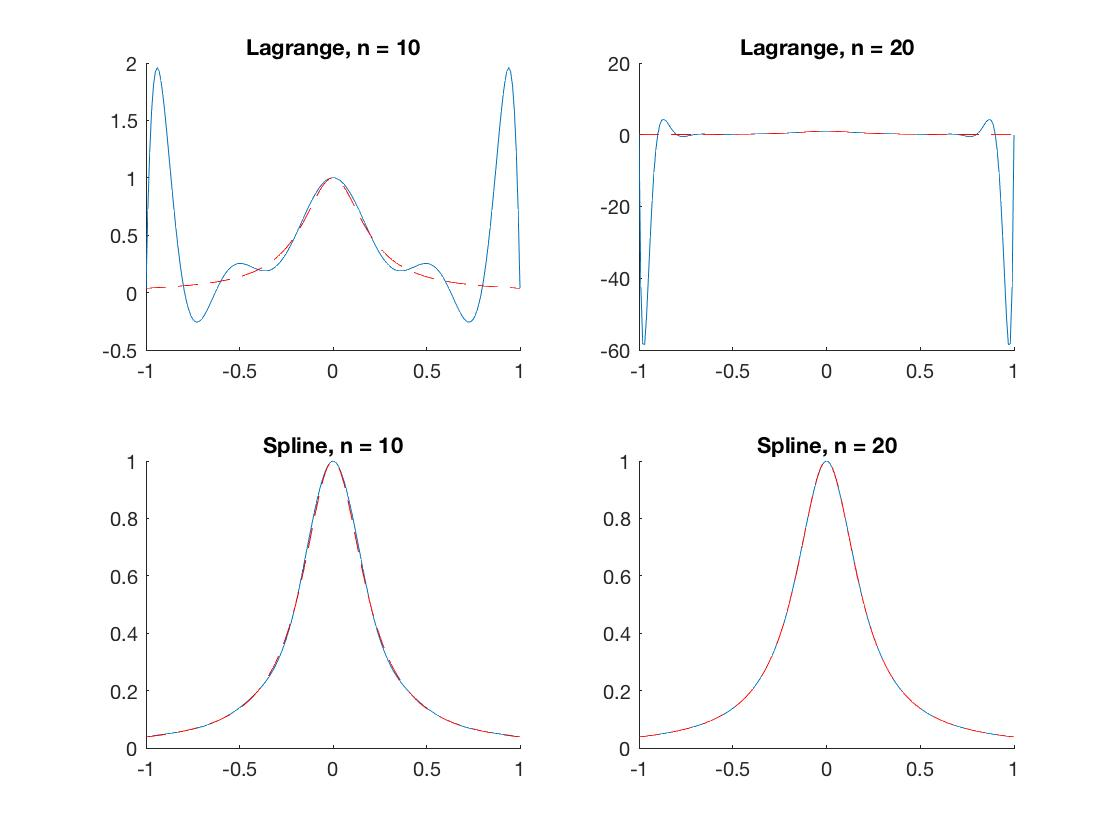
\includegraphics[height=9.9cm]{interp.jpg}
  \end{figure}
  \newpage
  \lstinputlisting{../Ex3_1.m}


\newpage
\section{补充练习}
\par\noindent1、基于spline求解其他两类边界条件对应的插值多项式。
  \lstinputlisting{../cubicSpline.m}

\end{document}
